% Báo cáo tìm hiểu hai công trình Multi-Agent Systems and Collaborative Reasoning
% Biên dịch bằng Tectonic (engine XeTeX) hoặc XeLaTeX/LuaLaTeX:
%   tectonic main.tex
% Font: Times New Roman của hệ thống (hỗ trợ đầy đủ tiếng Việt trên Windows);
% trên Linux/macOS hãy đổi sang TeX Gyre Termes trong phần fontspec bên dưới.
\documentclass[conference]{IEEEtran}
\IEEEoverridecommandlockouts

\usepackage{fontspec}
% --- Windows ---
\setmainfont{Times New Roman}
\setsansfont{Arial}
\setmonofont{Consolas}
% --- Linux/macOS (bỏ chú thích ba dòng dưới, chú thích ba dòng trên):
% \setmainfont{TeX Gyre Termes}
% \setsansfont{TeX Gyre Heros}
% \setmonofont{TeX Gyre Cursor}

\usepackage{amsmath,amssymb}
\usepackage{graphicx}
\usepackage{booktabs}
\usepackage{multirow}
\usepackage{url}
\usepackage[hidelinks]{hyperref}
\usepackage{xcolor}

% Ghi chú kết quả tự chạy — dùng để tách bạch số liệu của tác giả và số liệu tự đo
\newcommand{\ours}[1]{#1}

\title{Tìm hiểu và thực nghiệm các phương pháp cải thiện\\ giao tiếp và phối hợp tác tử trong hệ thống Multi-Agent}

\author{
\IEEEauthorblockN{Họ và tên sinh viên}
\IEEEauthorblockA{Khoa/lớp -- Trường Đại học\\
Email}
\and
\IEEEauthorblockN{Hướng dẫn: Giảng viên hướng dẫn}
\IEEEauthorblockA{Bộ môn}
}

\begin{document}
\maketitle

\begin{abstract}
Bài báo cáo này tìm hiểu hai công trình gần đây về giao tiếp và phối hợp tác tử trong hệ thống đa tác tử. Công trình thứ nhất, Agent-Radar, xử lý tình trạng lịch sử trao đổi phình to khiến thông tin liên quan bị loãng trong ngữ cảnh của các tác tử dựa trên LLM. Công trình này chấm điểm từng câu trong lịch sử theo độ tương đồng ngữ nghĩa nhân với hai hệ số suy giảm theo khoảng cách trên đồ thị giao tiếp và theo thời gian, rồi lái attention của mô hình về các câu được chọn mà không xóa bỏ gì. Công trình thứ hai, DAIN, coi việc hợp nhất dữ liệu đa phương thức là quá trình cộng tác giữa tám tác tử chuyên biệt: một Meta-Controller chỉ kích hoạt nhóm tác tử phù hợp với từng mẫu đầu vào và điều phối trao đổi thông tin nén giữa chúng. Báo cáo phân tích hai phương pháp, so sánh thiết kế của chúng, và xây dựng hai chương trình thực nghiệm có thể chạy lại: một thí nghiệm đánh giá chất lượng chọn ngữ cảnh của cơ chế Agent-Radar trên HotpotQA với lịch sử trao đổi mô phỏng, và một thí nghiệm huấn luyện bản DAIN đơn giản hóa trên dữ liệu thật ENRICO để so sánh với các baseline fusion tĩnh. Kết quả đo được cho thấy bộ chọn ngữ cảnh theo công thức của Agent-Radar nén lịch sử xuống khoảng 3\% số từ trong khi tăng mật độ bằng chứng gấp đôi, và thí nghiệm cũng cho thấy khi cơ chế này được dùng như bộ lọc cứng (không có bước lái attention như paper gốc) thì chất lượng trả lời của một bộ đọc yếu giảm xuống -- nhất quán với lập luận của chính paper rằng chọn ngữ cảnh phải đi kèm cách đưa nó vào lúc suy luận. Với DAIN, bản đơn giản hóa tái hiện đúng thứ tự ablation của paper (mô hình đầy đủ tốt hơn biến thể bỏ giao tiếp và biến thể bỏ điều phối) nhưng không tái hiện được lợi thế so với early fusion khi dữ liệu nhỏ và encoder yếu. Báo cáo cũng nêu rõ những phần chỉ là mô phỏng hoặc đơn giản hóa và những gì không thể kiểm chứng trong điều kiện tài nguyên hiện có.
\end{abstract}

\begin{IEEEkeywords}
Multi-Agent Systems, Collaborative Reasoning, Agent-Radar, DAIN, Agent Communication, Dynamic Agent Coordination
\end{IEEEkeywords}

\section{Giới thiệu}

Một hệ thống đa tác tử (Multi-Agent System -- MAS) dựa trên mô hình ngôn ngữ lớn (LLM) chia một nhiệm vụ khó cho nhiều tác tử, mỗi tác tử giữ một vai trò riêng và trao đổi kết quả trung gian với nhau. Cách làm này đạt hiệu quả cao trên nhiều tác vụ suy luận phức tạp, nhưng nó tạo ra một vấn đề đi kèm: các tác tử nói nhiều với nhau, và những gì chúng nói tích tụ thành ngữ cảnh rất dài. Khi lịch sử trao đổi dài ra, câu trả lời của một tác tử có thể phụ thuộc vào vài câu nhỏ nằm giữa hàng nghìn từ nhiễu. Hiện tượng mô hình bỏ sót thông tin nằm giữa ngữ cảnh dài đã được mô tả trong tài liệu với tên gọi ``lost in the middle''~\cite{liu2024lost}.

Hai bài báo được tìm hiểu trong báo cáo này tiếp cận vấn đề trên từ hai phía khác nhau. \textbf{Agent-Radar}~\cite{agentradar2026} xử lý phía \emph{đọc}: khi một tác tử chuẩn bị sinh câu trả lời, lịch sử trao đổi nên được đọc theo cách có chọn lọc thay vì đọc đều như nhau. Phương pháp này chấm điểm từng câu theo độ liên quan ngữ nghĩa, điều chỉnh theo khoảng cách giữa các tác tử trên đồ thị giao tiếp và theo tuổi của thông điệp, rồi lái attention của LLM về các câu được chọn. \textbf{DAIN}~\cite{dain2026} xử lý phía \emph{tham gia}: trong bài toán hợp nhất dữ liệu đa phương thức, không phải mọi chuyên gia đều cần chạy cho mọi mẫu đầu vào. DAIN dùng một bộ điều phối học được để kích hoạt thưa một nhóm tác tử chuyên biệt cho từng mẫu và điều phối trao đổi thông tin nén giữa chúng.

Hai công trình này được chọn vì chúng bổ sung cho nhau theo một hướng khá tự nhiên: một bên quản lý \emph{thông tin} luân chuyển giữa các tác tử, một bên quản lý \emph{thành phần} tham gia suy luận. Cả hai đều đưa ra cách chọn lọc phụ thuộc ngữ cảnh thay vì chính sách tĩnh, và cả hai đều có kết quả thực nghiệm chi tiết để đối chiếu.

Phạm vi của báo cáo giới hạn ở việc tìm hiểu và minh họa hai công trình nêu trên; đây là bài báo cáo học tập, không phải công trình đề xuất thuật toán mới. Cụ thể, báo cáo gồm các phần sau. Phần~\ref{sec:background} nhắc lại các khái niệm cần thiết. Phần~\ref{sec:agentradar} và phần~\ref{sec:dain} phân tích từng phương pháp. Phần~\ref{sec:comparison} so sánh hai thiết kế. Phần~\ref{sec:experiments} mô tả hai chương trình thực nghiệm, và phần~\ref{sec:results} trình bày kết quả đo được. Phần~\ref{sec:conclusion} kết luận.

\section{Cơ sở lý thuyết và công trình liên quan}\label{sec:background}

Phần này nhắc lại những khái niệm cần dùng khi đọc hai công trình chính, giữ ở mức vừa đủ để theo dõi các phần sau.

\subsection{Hệ đa tác tử dựa trên LLM và suy luận cộng tác}
Một hệ đa tác tử (MAS) gồm nhiều thực thể tự chủ, mỗi thực thể được trang bị một vai trò, một tập thông tin và một quy trình suy luận riêng. Với các LLM, ``tác tử'' thường được hiện thực bằng một prompt mô tả vai trò (ví dụ \emph{nhà phê bình}, \emph{chuyên gia toán học}) chạy trên cùng một mô hình nền. \emph{Suy luận cộng tác} (collaborative reasoning) là cách tổ chức trong đó các tác tử lần lượt sinh câu trả lời, đọc câu trả lời của nhau và chỉnh sửa theo nhiều vòng, ví dụ tranh luận đa tác tử (Multi-Agent Debate)~\cite{du2024debate} hay các khung như AutoGen~\cite{wu2024autogen} và GPTSwarm~\cite{zhuge2024gptswarm}. Lợi ích đến từ việc các tác tử bù thiếu sót cho nhau; cái giá là toàn bộ nội dung trao đổi đều nằm trong ngữ cảnh của những lần sinh sau.

\subsection{Giao tiếp tác tử và quản lý ngữ cảnh}
Trong MAS, \emph{giao tiếp} là quá trình một tác tử chuyển thông điệp cho tác tử khác theo một cấu trúc liên kết (topology) cho trước: liên kết đầy đủ, phân tầng, hoặc ngẫu nhiên. Lịch sử giao tiếp chính là ngữ cảnh đầu vào của các tác tử. \emph{Quản lý ngữ cảnh} (context management) là tập các kỹ thuật giữ cho ngữ cảnh hữu dụng khi nó dài ra: tóm tắt định kỳ, cắt tỉa thông điệp hoặc tác tử thừa (ví dụ AgentPrune~\cite{zhang2025agentprune} và AgentDropout~\cite{wang2025agentdropout}), hoặc -- như Agent-Radar -- giữ nguyên lịch sử và thay đổi cách chú ý tới nó.

\subsection{Attention steering}
Cơ chế attention của Transformer cho phép mô hình gán trọng số cho từng vị trí trong ngữ cảnh khi sinh từ tiếp theo~\cite{vaswani2017attention}. \emph{Attention steering} là nhóm kỹ thuật can thiệp trực tiếp vào cơ chế này ở lúc suy luận: khuếch đại attention vào một đoạn được chỉ định (Selective Prompt Anchoring -- SPA~\cite{tian2025spa}, PASTA~\cite{zhang2024pasta}). Đặc điểm chung của nhóm này là không cần huấn luyện lại, nhưng cần truy cập vào bên trong mô hình, nên chỉ áp dụng được với LLM chạy cục bộ.

\subsection{Hợp nhất đa phương thức và Mixture-of-Experts}
\emph{Hợp nhất đa phương thức} (multimodal fusion) là bài toán kết hợp thông tin từ nhiều loại dữ liệu -- ảnh, văn bản, âm thanh, dữ liệu chuỗi -- để ra một dự đoán. Khung \emph{Partial Information Decomposition}~\cite{liang2023pid} chia thông tin liên modality thành ba loại: thông tin riêng của từng modality (uniqueness), thông tin trùng nhau giữa các modality (redundancy) và thông tin chỉ xuất hiện khi kết hợp (synergy). Kiến trúc \emph{Mixture-of-Experts} (MoE)~\cite{jacobs1991adaptive} dùng nhiều mạng con ``chuyên gia'' và một bộ định tuyến chọn cách trộn đầu ra của chúng theo từng mẫu; phiên bản thưa (sparse MoE)~\cite{shazeer2017outrageously} chỉ chạy một nhóm chuyên gia nhỏ cho mỗi mẫu. DAIN kế thừa cả hai ý trên nhưng thay bộ định tuyến tĩnh bằng một bộ điều phối học được kèm trao đổi thông tin giữa các chuyên gia.

\subsection{Điều phối động tác tử}
\emph{Điều phối động} (dynamic coordination) nghĩa là nhóm tác tử tham gia và đường thông tin giữa chúng được quyết định theo từng đầu vào, khác với kiến trúc tĩnh trong đó mọi tác tử chạy với cùng một sơ đồ. Hai hình thức động gặp trong hai paper: chọn lại ngữ cảnh ở mỗi bước sinh (Agent-Radar) và chọn lại nhóm tác tử cho mỗi mẫu (DAIN).

\section{Phương pháp Agent-Radar}\label{sec:agentradar}

\subsection{Bài toán và động lực nghiên cứu}
Trong một hệ MAS dựa trên LLM, mỗi vòng trao đổi thêm một lớp thông điệp vào ngữ cảnh của mọi tác tử liên quan. Sau vài vòng, ngữ cảnh của một tác tử chứa rất nhiều thứ: câu hỏi gốc, các ràng buộc của nhiệm vụ, bằng chứng trung gian hữu dụng, và một lượng lớn câu lặp ý hoặc lạc đề. Mô hình phải ``tìm đúng'' vài câu quan trọng trong đống này, và theo~\cite{liu2024lost}, khả năng tìm đúng giảm rõ khi thông tin nằm giữa ngữ cảnh dài. Agent-Radar nêu ra hai hướng xử lý phổ biến trước đó đều có nhược điểm chung: tóm tắt định kỳ nén lịch sử nhưng có thể bỏ mất tín hiệu tinh tế; cắt tỉa tác tử hoặc liên kết giảm token nhưng vĩnh viễn bỏ đi một phần thông tin~\cite{agentradar2026}.

\subsection{Ý tưởng cốt lõi}
Agent-Radar chọn hướng thứ ba: \emph{không xóa, không nén, không sửa lịch sử}. Thay vào đó, với mỗi bước sinh của mỗi tác tử, phương pháp chọn ra một tập câu liên quan trong lịch sử và lái attention của LLM về tập đó. Toàn bộ lịch sử vẫn nằm trong prompt; các câu được chọn chỉ nhận thêm ``sự chú ý''. Vì vậy phương pháp là một lớp phủ (plug-in) training-free: không cần huấn luyện, không đổi topology của hệ MAS, không đổi trọng số LLM.

\subsection{Công thức hóa và kiến trúc}
Paper mô hình hóa hệ MAS là đồ thị có hướng $G = (V, E, F)$, với $V$ là tập $N$ tác tử, $E$ là tập cạnh giao tiếp, $F$ là tập hàm suy luận~\cite{agentradar2026}. Khoảng cách giữa hai tác tử $d_G(v_j, v_i)$ là số cạnh của đường đi ngắn nhất từ $v_j$ đến $v_i$. Tại vòng $t$, tác tử đang hoạt động $v_i$ sinh phản hồi
\begin{equation}
o^{(t)}_i = f_i\big(q^{(t)}, Z^{(t)}_i\big),
\label{eq:ar-infer}
\end{equation}
trong đó $q^{(t)}$ là truy vấn hiện tại và $Z^{(t)}_i$ là lịch sử tích lũy từ mọi tác tử tới được $v_i$. Agent-Radar bổ sung tham số $\hat{Z}^{(t)}_i$ -- ngữ cảnh được chọn -- và cập nhật bước suy luận thành $o^{(t)}_i = f_i(q^{(t)}, Z^{(t)}_i, \hat{Z}^{(t)}_i)$.

\subsection{Cơ chế đánh giá mức liên quan của ngữ cảnh}
Mỗi thông điệp $o^{(\tau)}_j$ trong lịch sử nhận một điểm liên quan gồm hai nhân tử suy giảm:
\begin{equation}
r_i(o^{(\tau)}_j; t) = \underbrace{\lambda_s^{\,d_G(v_j, v_i) - 1}}_{\text{suy giảm không gian}} \cdot \underbrace{\lambda_t^{\,t - \tau - 1}}_{\text{suy giảm thời gian}},
\label{eq:ar-decay}
\end{equation}
với $0 < \lambda_s, \lambda_t < 1$. Thông điệp từ tác tử là láng giềng trực tiếp (hoặc của chính tác tử) có trọng số không gian bằng 1; thông điệp mới nhất có trọng số thời gian bằng 1. Ý nghĩa của hai nhân tử khác nhau: $\lambda_s$ nói rằng thông tin đi qua càng nhiều trung gian càng khó tin và dễ nhiễu; $\lambda_t$ nói rằng thông tin càng cũ càng có khả năng đã bị sửa hoặc thay thế ở các vòng sau.

Trên nền hai hệ số đó, paper thực hiện truy xuất mức câu. Mỗi thông điệp được cắt thành các câu $s_k$, mã hóa bằng một sentence encoder (all-MiniLM-L6-v2~\cite{reimers2019sbert}), và so cosine với truy vấn hiện tại. Điểm tổng hợp của câu $s_k$ là
\begin{equation}
\mathrm{score}(s_k) = r_i(o^{(\tau)}_j; t)\cdot \cos\big(\mathrm{Enc}(s_k), \mathrm{Enc}(q^{(t)})\big).
\label{eq:ar-score}
\end{equation}
Ngữ cảnh được chọn gồm truy vấn và mọi câu có điểm vượt ngưỡng $\theta$:
\begin{equation}
\hat{Z}^{(t)}_i = \{q^{(t)}\} \cup \big\{s_k \mid \mathrm{score}(s_k) \ge \theta\big\}.
\label{eq:ar-select}
\end{equation}
Truy vấn luôn được giữ lại, để phần lịch sử được chọn không lấn át mục tiêu suy luận. Thiết lập mặc định của paper: $\lambda_s = \lambda_t = 0{,}92$ và $\theta = 0{,}65$.

\subsection{Cơ chế lái attention}
Các câu trong $\hat{Z}^{(t)}_i$ được khuếch đại attention bằng Selective Prompt Anchoring (SPA)~\cite{tian2025spa}, một kỹ thuật can thiệp vào phân bố logit tại lúc suy luận, không đụng vào trọng số mô hình. Paper cũng thử thay SPA bằng PASTA~\cite{zhang2024pasta} và thấy phương pháp vẫn có lợi, nên cơ chế này không phụ thuộc một backend cụ thể.

\emph{Ví dụ nhỏ.} Giả sử tác tử đang đọc ở vòng $t=4$, truy vấn hỏi về một khái niệm tổ chức. Một câu từ báo cáo của tác tử láng giềng (hop $=1$) ở vòng 3 có điểm suy giảm $\lambda_s^0 \cdot \lambda_t^0 = 1$; nếu cosine với truy vấn là $0{,}8$ thì score là $0{,}8 \ge \theta$ -- được chọn. Một câu nội dung tương tự nhưng từ tác tử cách 3 hop và viết ở vòng 1 có điểm $\lambda_s^2 \cdot \lambda_t^2 \cdot 0{,}8 \approx 0{,}51$ -- không qua ngưỡng, dù câu vẫn nằm nguyên trong lịch sử.

\subsection{Thiết lập thực nghiệm trong paper}
Agent-Radar được đánh giá trên năm bộ dữ liệu: HotpotQA, 2WikiMultihopQA, MuSiQue (báo cáo F1), MATH-500 và MMLU-Pro (báo cáo accuracy). Mô hình nền chính là Qwen3-4B-Instruct, kiểm chứng thêm trên Llama-3.1-8B và Qwen3-32B. Hệ MAS mặc định gồm 5 tác tử chạy 2 vòng trên đồ thị ngẫu nhiên; baseline gồm Vanilla, CoT-SC, Compaction (nén ngữ cảnh), AgentPrune và AgentDropout (cắt tỉa). Phương pháp cũng được cắm vào ba khung MAS có sẵn: GPTSwarm, AutoGen và MAD.

\subsection{Kết quả và nhận xét}
Số liệu trong phần này là kết quả do các tác giả của Agent-Radar công bố~\cite{agentradar2026}. Trên cả năm bộ dữ liệu, Agent-Radar đạt điểm cao nhất trong số các phương pháp so sánh: 80,78 F1 trên HotpotQA (+7,64 so với AgentDropout, mức tăng lớn nhất được nêu), 80,81 trên 2Wiki, 39,72 trên MuSiQue, 88,80 trên MATH-500 và 69,40 trên MMLU-Pro. Khi cắm vào GPTSwarm, mức tăng lớn nhất là 12,87 điểm F1 trên MuSiQue. Phương pháp giữ lợi thế trên cả topology phân tầng và liên kết đầy đủ.

Hai kết quả ablation đáng chú ý. Thứ nhất, bỏ phần lái attention (chỉ nối thêm các câu được chọn vào prompt) làm MuSiQue giảm từ 39,72 xuống 35,27 -- nghĩa là chọn ngữ cảnh tốt thôi chưa đủ, cách đưa nó vào lúc suy luận cũng quan trọng. Thứ hai, bỏ riêng suy giảm không gian làm MuSiQue giảm xuống 28,41, mạnh hơn cả việc bỏ đồng thời hai hệ số suy giảm (33,97); tác giả giải thích rằng chỉ dùng một trong hai hệ số có thể đẩy sai lệch điểm số theo một chiều, trong khi kết hợp cả hai mới phân biệt được bằng chứng thật với nhiễu. Về chi phí, thời gian chạy tăng từ 968,8 lên 1196,5 giây mỗi nhiệm vụ (khoảng +23\%), thấp hơn mức tăng của Compaction và AgentDropout.

Giới hạn được nêu trong paper: cần chọn $\lambda_s, \lambda_t, \theta$ bằng tay; chất lượng phụ thuộc bộ truy xuất ngữ nghĩa; và phải có backend can thiệp attention, vốn chỉ hoạt động với LLM chạy cục bộ.

\section{Phương pháp DAIN}\label{sec:dain}

\subsection{Bài toán suy luận đa phương thức}
Bài toán ở đây khác Agent-Radar về bản chất: đầu vào của mô hình gồm nhiều modality (ảnh, văn bản, âm thanh, dữ liệu lâm sàng...), và việc hợp nhất chúng quyết định chất lượng dự đoán. Các kiến trúc fusion phổ biến -- nối đặc trưng (early fusion), hợp nhất dự đoán (late fusion), hoặc các biến thể MoE -- đều có cấu trúc cố định: mọi modality, mọi ``chuyên gia'' chạy theo cùng một sơ đồ cho mọi mẫu. DAIN lập luận rằng các tương tác giữa modality chia làm ba loại theo khung PID~\cite{liang2023pid} (uniqueness, redundancy, synergy), và với từng mẫu cụ thể chỉ một số loại tương tác là cần thiết; chạy toàn bộ vừa tốn vừa nhét nhiễu vào dự đoán.

\subsection{Ý tưởng điều phối tác tử động}
DAIN chuyển bài toán fusion thành bài toán cộng tác đa tác tử: một pool các \emph{tác tử tương tác} chuyên biệt, mỗi tác tử phụ trách một loại tương tác đa phương thức, và một \emph{Meta-Controller} quyết định -- cho từng mẫu -- tác tử nào chạy và chúng trao đổi thông tin với nhau theo đường nào. Khác MoE thông thường, các tác tử được chọn còn trao đổi thông tin với nhau trước khi hợp nhất, và toàn bộ quá trình (điều phối, giao tiếp, hợp nhất) học cùng nhau từ đầu đến cuối.

\subsection{Kiến trúc DAIN}
Kiến trúc gồm ba giai đoạn~\cite{dain2026}. Pool có $K = 8$ tác tử, chia theo PID thành 3 tác tử synergy, 3 tác tử uniqueness và 2 tác tử redundancy (phân bổ này có thể đổi theo nhiệm vụ). Mỗi modality $m_i$ được mã hóa bởi một encoder riêng $E_i$ thành embedding $e_i$.

Giai đoạn đầu, Meta-Controller tạo vector ngữ cảnh bằng cách nối các embedding và chiếu tuyến tính:
\begin{equation}
e_c = W_c[e_1; e_2; \dots; e_n] + b_c.
\label{eq:dain-ctx}
\end{equation}
Từ $e_c$, bộ điều phối sinh vector kích hoạt thưa:
\begin{equation}
g = \mathrm{Top}_\tau\big(\mathrm{Softmax}(G_{gate}(e_c))\big),
\label{eq:dain-gate}
\end{equation}
chỉ giữ $\tau$ tác tử có gate khác 0, và đồng thời sinh đồ thị giao tiếp mềm
\begin{equation}
\Phi = \sigma\big(G_{comm}(e_c)\big) \in \mathbb{R}^{K\times K},
\label{eq:dain-comm}
\end{equation}
trong đó $\Phi_{ij}$ là độ mạnh dòng thông tin từ tác tử $A_j$ sang $A_i$. Cả hai đều phụ thuộc từng mẫu đầu vào.

Giai đoạn hai, mỗi tác tử được kích hoạt tính trạng thái ban đầu $h^{(0)}_k = f_k(e_c;\theta_k)$, rồi trao đổi thông tin qua một nút cổ chai nén: thông điệp từ $A_j$ tới $A_i$ là $m_{i\leftarrow j} = B(h^{(0)}_j;\,\phi_{ij})$ với $\phi_{ij} = \Phi_{ij}\cdot\mathbb{I}(g_j > 0)$ và $B(h;\phi) = \phi\,(W_B h)$, trong đó $W_B$ là phép chiếu hạng thấp. Kết nối mạnh cho truyền nhiều thông tin; kết nối yếu gần như chặn. Trạng thái sau trao đổi là
\begin{equation}
h^{(1)}_i = \mathrm{LayerNorm}\Big(h^{(0)}_i + \mathrm{ReLU}\Big(W_u \textstyle\sum_{j\neq i} m_{i\leftarrow j}\Big)\Big).
\label{eq:dain-update}
\end{equation}
Giai đoạn ba, dự đoán được hợp nhất bằng một module multi-head attention trên trạng thái của các tác tử đang bật: $\hat{y} = C(\{h^{(1)}_k \mid g_k > 0\})$.

\subsection{Vai trò của Meta-Controller}
Meta-Controller gánh hai quyết định trong một lần tính: \emph{ai chạy} (Eq.~\ref{eq:dain-gate}) và \emph{ai nói với ai} (Eq.~\ref{eq:dain-comm}). Cả hai chỉ đọc vector ngữ cảnh $e_c$, nên chi phí điều phối nhỏ (0,26 triệu tham số trong triển khai của paper) so với phần còn lại của mô hình. Nhờ điều phối theo mẫu, mô hình có thể ``dài ra'' bằng cách thêm tác tử vào pool mà không tăng chi phí tuyến tính theo số tác tử cho mỗi mẫu.

\subsection{Hàm mục tiêu và các thành phần tối ưu hóa}
DAIN huấn luyện với hàm loss tổng hợp:
\begin{equation}
L_{total} = L_{task} + \alpha L_{spec} + \lambda_{act}\|g\|_1 + \lambda_{comm}\|\Phi\|_F^2,
\label{eq:dain-loss}
\end{equation}
trong đó $L_{task}$ là cross-entropy (phân loại) hoặc MSE (hồi quy). Thành phần chuyên môn hóa $L_{spec}$ đo độ phân kỳ của đầu ra từng tác tử khi làm nhiễu đầu vào (che từng modality): một tác tử thật sự chuyên môn phải phản ứng khác nhau khi mất các modality khác nhau. Hai số hạng còn lại điều tiết hiệu suất: $\|g\|_1$ ép kích hoạt thưa hơn mức $\tau$ cho phép, $\|\Phi\|_F^2$ chống đồ thị giao tiếp dày đặc. Paper cũng nêu phân tích hội tụ $O(1/\sqrt{T})$ và chi phí tính toán $O(\bar{\tau} C_{agent} + \bar{\tau}^2 C_{comm})$ với $\bar{\tau}$ là số tác tử kích hoạt trung bình.

\subsection{Thiết lập thực nghiệm trong paper}
Số liệu trong phần này là kết quả do các tác giả của DAIN công bố~\cite{dain2026}. Đánh giá trên năm bộ dữ liệu đa phương thức: ADNI (chẩn đoán Alzheimer từ MRI, PET, dữ liệu gen), MIMIC-IV (dự báo tử vong ICU), MM-IMDB (phân loại thể loại phim từ poster và tóm tắt), CMU-MOSI (cường độ cảm xúc từ video, âm thanh, văn bản) và ENRICO (phân loại chủ đề thiết kế màn hình di động). Encoder là ResNet-50 (ảnh), BERT-base (văn bản) và transformer cho dữ liệu chuỗi, embedding 512 chiều. Huấn luyện bằng Adam, lr $10^{-4}$, batch 32, early stopping patience 10; $\alpha = 0{,}1$, $\lambda_{act} = 0{,}01$, $\lambda_{comm} = 0{,}001$; mỗi cấu hình chạy 5 seed và báo cáo trung bình $\pm$ độ lệch chuẩn.

\subsection{Kết quả và nhận xét}
DAIN đạt kết quả cao nhất trên cả năm bộ dữ liệu, với mức tăng so với baseline tốt nhất là +2,6\% accuracy trên ADNI, +1,7\% trên MIMIC-IV, +2,1\% trên MM-IMDB, $-0{,}07$ MSE trên MOSI và +1,3\% trên ENRICO (đều $p<0{,}001$). Về hiệu suất, mô hình 12,8 triệu tham số nhưng mỗi lượt suy luận chỉ dùng trung bình 5,8 triệu nhờ kích hoạt thưa; số tác tử kích hoạt trung bình $\bar{\tau}$ dao động từ 3,2 đến 5,5 trên tổng 8, và mật độ đồ thị giao tiếp $\bar{\rho}$ từ 0,19 đến 0,42 tùy bộ dữ liệu.

Ablation xác nhận vai trò của hai thành phần chính: bỏ điều phối động (mọi tác tử luôn bật -- DAIN-Static) làm ADNI giảm 1,7 điểm; bỏ trao đổi thông tin (DAIN-NoComm) giảm 1,4 điểm; trong khi MoE tĩnh cùng quy mô thấp hơn DAIN tới 3,4 điểm. Khi quét $\tau$, hiệu quả đạt đỉnh ở $\tau = 4$ rồi giảm nhẹ -- nhiều tác tử hơn không giúp gì vì các tác tử thừa chỉ thêm nhiễu. Phân tích khả năng diễn giải cho thấy các nhóm tác tử được dùng theo đúng trực giác dữ liệu: bệnh nhân nhận thức bình thường (ADNI) kích hoạt mạnh nhóm uniqueness, còn bệnh nhân MCI/Dementia kích hoạt mạnh nhóm synergy; thể loại phim dựa trên hình ảnh riêng biệt (Animation) dùng uniqueness, thể loại kết hợp hình ảnh và cốt truyện (Thriller) dùng synergy.

Paper nêu bốn giới hạn: phân bổ nhóm tác tử là thủ công; Meta-Controller thêm chi phí không đáng kể với mô hình lớn nhưng có thể thành gánh nặng với mô hình nền rất nhẹ; đánh giá mới dừng ở phân loại và hồi quy; và mô hình kích hoạt tác tử là dữ kiện gợi ý chứ chưa phải giải thích hình thức.

\section{So sánh và thảo luận}\label{sec:comparison}

\begin{table*}[t]
\centering
\caption{So sánh tổng quan hai công trình. Số liệu hiệu năng lấy từ paper gốc của từng phương pháp; hai phương pháp không đánh giá trên cùng bộ dữ liệu nên không so điểm trực tiếp.}
\label{tab:compare}
\begin{tabular}{p{0.20\textwidth} p{0.35\textwidth} p{0.35\textwidth}}
\toprule
\textbf{Tiêu chí} & \textbf{Agent-Radar}~\cite{agentradar2026} & \textbf{DAIN}~\cite{dain2026} \\
\midrule
Mục tiêu & Cải thiện cách tác tử LLM tận dụng lịch sử trao đổi dài & Cải thiện hợp nhất đa phương thức cho suy luận cộng tác \\
Loại bài toán & Quản lý ngữ cảnh lúc suy luận trong MAS & Fusion đa phương thức học được (phân loại, hồi quy) \\
Kiến trúc & Lớp phủ chọn ngữ cảnh + lái attention trên MAS có sẵn & Mạng nơ-ron hoàn chỉnh: Meta-Controller, pool 8 tác tử, đồ thị giao tiếp, consensus fusion \\
Cơ chế giao tiếp & Không đổi cách tác tử giao tiếp; thay đổi cách một tác tử đọc lại lịch sử & Trao đổi nén qua nút cổ chai $B(h;\phi)=\phi W_B h$, đồ thị $\Phi$ theo từng mẫu \\
Cách chọn & Chọn \emph{câu}: cosine ngữ nghĩa $\times$ suy giảm không gian (hop) $\times$ thời gian (tuổi), ngưỡng $\theta$ & Chọn \emph{tác tử}: top-$\tau$ gate theo ngữ cảnh; chọn \emph{luồng thông tin}: $\Phi=\sigma(G_{comm}(e_c))$ \\
Yêu cầu huấn luyện & Training-free (chỉ cần sentence encoder có sẵn) & Huấn luyện từ đầu, loss đa mục tiêu (Eq.~\ref{eq:dain-loss}) \\
Chi phí & $+23\%$ thời gian mỗi nhiệm vụ; lịch sử đầy đủ vẫn nằm trong prompt & 12,8M tham số tổng, 5,8M dùng mỗi lượt nhờ kích hoạt thưa \\
Bộ dữ liệu đánh giá & HotpotQA, 2Wiki, MuSiQue, MATH-500, MMLU-Pro (văn bản) & ADNI, MIMIC-IV, MM-IMDB, CMU-MOSI, ENRICO (đa phương thức) \\
Ưu điểm & Không mất thông tin, cắm được vào nhiều khung MAS, không cần huấn luyện & Tiết kiệm tính toán theo mẫu, diễn giải được qua mô hình kích hoạt \\
Giới hạn & Cần backend can thiệp attention (SPA/PASTA) chỉ chạy với LLM cục bộ; chỉnh tay $\lambda_s,\lambda_t,\theta$ & Phân bổ nhóm tác tử thủ công; mới cho phân loại/hồi quy; cần huấn luyện từ đầu \\
\bottomrule
\end{tabular}
\end{table*}

Bảng~\ref{tab:compare} đối chiếu hai công trình theo từng tiêu chí. Phần dưới phân tích những điểm giống, khác và những gì rút ra được khi đọc cả hai.

\subsection{Điểm tương đồng}
Hai paper phản ứng với cùng một vấn đề chung: khi số thành phần tham gia cộng tác tăng lên -- nhiều tác tử, nhiều vòng, nhiều modality -- việc để mọi thành phần truy cập hoặc xử lý \emph{mọi thứ} vừa tốn kém vừa làm giảm chất lượng. Agent-Radar cắt gọn vấn đề ở mức thông tin: không phải câu nào trong lịch sử cũng xứng đáng nhận attention như nhau. DAIN cắt gọn ở mức thành phần: không phải tác tử nào cũng cần chạy cho mọi mẫu. Hai hướng chạm nhau ở một nguyên tắc: \emph{lựa chọn phụ thuộc ngữ cảnh} -- Agent-Radar tính điểm cho từng câu theo truy vấn hiện tại, DAIN tính gate cho từng tác tử theo vector ngữ cảnh của từng mẫu -- thay vì dùng chính sách tĩnh áp cho mọi tình huống.

Nguyên tắc thứ hai cả hai cùng dùng là \emph{khoảng cách cấu trúc là tín hiệu hữu ích}. Agent-Radar đo khoảng cách hop trên đồ thị giao tiếp và suy giảm trọng số theo nó; DAIN học luôn đồ thị giao tiếp $\Phi$. Trong cả hai paper, bỏ yếu tố cấu trúc này đều làm kết quả xấu đi rõ rệt: bỏ suy giảm không gian làm MuSiQue giảm từ 39,72 xuống 28,41 trong Agent-Radar; bỏ trao đổi giữa các tác tử làm ADNI giảm từ 73,5 xuống 72,1 trong DAIN (số liệu tác giả).

Thứ ba, cả hai đều tránh cắt cụt mù. Agent-Radar giữ nguyên toàn bộ lịch sử và chỉ lái attention; DAIN nén thông điệp qua nút cổ chai với độ mạnh tỷ lệ độ mạnh kết nối, thay vì chặn hẳn tin nhắn.

\subsection{Khác biệt quan trọng}
Khác biệt đầu tiên nằm ở tầng hoạt động. Agent-Radar là kỹ thuật lúc suy luận cho một hệ đã có: không có tham số cần huấn luyện, không đổi gì cấu trúc. DAIN là một kiến trúc học từ đầu: mọi cơ chế của nó -- gate, đồ thị giao tiếp, cách hợp nhất -- được hình thành trong huấn luyện. Vì thế không thể nói phương pháp nào ``tốt hơn'' bằng cách so điểm: chúng chạy trên loại dữ liệu khác nhau, loại tác vụ khác nhau và không chia sẻ baseline nào.

Khác biệt thứ hai là ý nghĩa của từ ``động''. Trong Agent-Radar, động là việc ngữ cảnh được chọn lại ở \emph{mỗi bước sinh của từng tác tử}. Trong DAIN, động là việc nhóm tác tử và đồ thị giao tiếp được tính lại cho \emph{mỗi mẫu}. Độ mịn của lựa chọn khác nhau: một bên chọn câu, một bên chọn thành phần mô hình.

Khác biệt thứ ba là hướng tối ưu tài nguyên, và hai phương pháp đi ngược chiều nhau. Agent-Radar \emph{tăng} chi phí suy luận khoảng 23\% để đổi lấy chất lượng, vì toàn bộ lịch sử vẫn nằm trong prompt và còn thêm phần chấm điểm câu. DAIN \emph{giảm} chi phí vì thành phần không được chọn thì không chạy (5,8M trên 12,8M tham số hiệu dụng). Ai muốn chọn một trong hai hướng nên bắt đầu từ câu hỏi: bài toán đang thiếu chất lượng hay đang thiếu tài nguyên.

Một điểm cần nói thẳng: Agent-Radar phụ thuộc khả năng can thiệp vào attention bên trong LLM (SPA, PASTA). Với các LLM chỉ gọi qua API, lớp kỹ thuật này không áp dụng được; đây là ràng buộc thực dụng mà paper xử lý bằng các mô hình cục bộ.

\subsection{Bài học thiết kế chung}
Đọc cả hai công trình, có thể rút ra vài nguyên tắc có vẻ lặp lại được ở các hệ khác. Thứ nhất, lựa chọn nên được tính từ đặc điểm tình huống (truy vấn, mẫu đầu vào) chứ không cố định trước. Thứ hai, cấu trúc liên kết giữa các thành phần -- kể cả khi nó đơn giản như số hop trên đồ thị -- mang thông tin về độ tin cậy của thông tin và nên được đưa vào quyết định chọn lọc. Thứ ba, cơ chế nén có kiểm soát (giữ nguyên bản gốc và lái sự chú ý, hoặc nén theo độ mạnh kết nối) giảm rủi ro mất thông tin so với việc xóa trực tiếp. Cuối cùng, mỗi cơ chế chọn lọc cần một ``van điều tiết'' chi phí -- ngưỡng $\theta$ ở Agent-Radar, các số hạng chính quy $\|g\|_1$ và $\|\Phi\|_F^2$ ở DAIN -- để cân bằng giữa độ phủ và chi phí.

\subsection{Khả năng kết hợp (giả thuyết, chưa được kiểm chứng)}
Về nguyên tắc có thể hình dung một hệ mà DAIN điều phối các tác tử LLM (chọn ai chạy cho mỗi nhiệm vụ) và Agent-Radar quản lý ngữ cảnh mà mỗi tác tử đọc lại giữa các vòng (chọn đọc gì). Đây chỉ là suy nghĩ thiết kế của người viết báo cáo: hai paper không thử nghiệm kết hợp này, hai cơ chế nằm ở tầng khác nhau, và việc chúng bù hay chéo nhau là câu hỏi mở cần thí nghiệm riêng.

\section{Thiết kế và triển khai thực nghiệm}\label{sec:experiments}

\subsection{Mục tiêu thực nghiệm}
Phần này trả lời câu hỏi: với tài nguyên thông thường (máy cá nhân, không GPU lớn, không gọi API LLM trả phí), có thể kiểm chứng được những gì từ hai paper?

Đối với Agent-Radar, việc tái hiện đúng thí nghiệm gốc là không khả thi: cần chạy LLM cục bộ quy mô 4--32B tham số với backend can thiệp attention (SPA) trên năm bộ benchmark. Phần có thể làm trung thực là \emph{cơ chế chọn ngữ cảnh} (Eq.~\ref{eq:ar-decay}--\ref{eq:ar-select}): các công thức này tự chứa, không cần LLM, chỉ cần một sentence encoder. Vì vậy thí nghiệm 1 đánh giá chất lượng của bộ chọn ngữ cảnh -- không đánh giá hiệu ứng lái attention lên câu trả lời của LLM. Mọi kết quả của thí nghiệm này được trình bày với tư cách \emph{phiên bản minh họa}, không phải tái hiện Agent-Radar.

Đối với DAIN, kiến trúc lõi (Eq.~\ref{eq:dain-ctx}--\ref{eq:dain-loss}) là một mô hình nhỏ có công thức tường minh nên có thể hiện thực và huấn luyện được. Phần không thể làm là encoder gốc (ResNet-50, BERT-base) và bốn trong năm bộ dữ liệu gốc (ADNI, MIMIC-IV cần đăng ký; MOSI cần đặc trưng cỡ lớn). Thí nghiệm 2 vì vậy là \emph{bản đơn giản hóa trung thực}: giữ nguyên cấu trúc thuật toán, thay encoder bằng bản nhẹ, chạy trên một bộ dữ liệu thật duy nhất (ENRICO) trong năm bộ của paper.

\subsection{Môi trường và thư viện}
Mọi thí nghiệm chạy trên một máy cá nhân: Windows 11, Python 3.13, CPU, không dùng GPU. Thư viện: torch 2.14 (huấn luyện), sentence-transformers (all-MiniLM-L6-v2 -- đúng encoder mà Agent-Radar dùng), scikit-learn, pandas, matplotlib. Toàn bộ mã nguồn, cấu hình và seed nằm trong thư mục \texttt{experiments/} của dự án; hướng dẫn chạy lại trong \texttt{README.md}. Đơn vị đo thời gian là giờ đồng hồ trên máy này và chỉ mang ý nghĩa so sánh tương đối giữa các chiến lược.

\subsection{Bộ dữ liệu}
\textbf{HotpotQA}~\cite{yang2018hotpotqa} (bản distractor, tập validation): mỗi mẫu gồm một câu hỏi, mười đoạn văn Wikipedia (2 đoạn chứa đáp án, 8 đoạn gây nhiễu) và danh sách supporting facts chỉ ra chính xác các câu chứa bằng chứng vàng. Nhãn câu-vàng cho phép đo chính xác mức độ ``giữ đúng thông tin'' của từng chiến lược chọn ngữ cảnh. Lấy 200 mẫu theo seed cố định.

\textbf{ENRICO}~\cite{leiva2020enrico}: 1460 màn hình ứng dụng di động, mỗi màn hình có ảnh chụp và cây phân cấp giao diện (chứa tên lớp, resource-id và nội dung văn bản của các thành phần UI), được gán một trong 20 chủ đề thiết kế. Độ nhỏ và tính công khai của bộ dữ liệu này khiến nó phù hợp để huấn luyện lặp lại nhiều seed trên CPU. Chia 70/10/20 phân tầng theo nhãn với seed cố định (không xác minh được đúng split gốc mà DAIN dùng).

\subsection{Các phương pháp đối chứng}
Thí nghiệm 1 so bốn chiến lược chọn ngữ cảnh, xếp theo mức gần với paper: (i) \texttt{full} -- giữ toàn bộ lịch sử, tương ứng baseline của hệ MAS không quản lý ngữ cảnh; (ii) \texttt{window} -- chỉ giữ vòng trao đổi gần nhất; (iii) \texttt{semantic} -- chỉ lọc theo cosine ngữ nghĩa với ngưỡng $\theta$, tương ứng biến thể ablation ``bỏ cả hai hệ số suy giảm'' trong Table~4 của paper; (iv) \texttt{radar} -- đúng công thức Eq.~\ref{eq:ar-decay}--\ref{eq:ar-select} với $\lambda_s=\lambda_t=0{,}92$, $\theta=0{,}65$ (giá trị mặc định của paper), tên gọi là \emph{phiên bản minh họa} vì thiếu thành phần lái attention.

Thí nghiệm 2 so bảy mô hình: Early Fusion, Late Fusion, Static MoE, Sparse MoE (cùng pool 8 expert), và ba biến thể DAIN -- DAIN-Static (mọi tác tử luôn bật), DAIN-NoComm (không trao đổi), DAIN đầy đủ -- đúng cấu trúc ablation trong Table~4 của paper DAIN. Baseline MMoE không chạy vì với một nhiệm vụ duy nhất MMoE suy biến về Static MoE (MMoE khác ở việc mỗi nhiệm vụ có một gate riêng).

\subsection{Quy trình triển khai}
\textbf{Thí nghiệm 1} (tệp \texttt{src/exp1/}): với mỗi mẫu HotpotQA, mô phỏng $P$ tác tử trao đổi trong $T$ vòng trên đồ thị ngẫu nhiên. Thông điệp của một tác tử gồm: (a) \emph{tín hiệu} -- câu vàng, mà các tác tử ``chuyên gia'' tự truy xuất được, còn tác tử thường chỉ lặp lại được những gì nghe từ láng giềng ở vòng trước (xác suất 0,5); (b) \emph{nhiễu} -- các câu từ đoạn gây nhiễu, số lượng tăng theo vòng ($3+t$ câu), mô phỏng hiện tượng lịch sử loãng dần mà paper mô tả. Nhãn vàng của từng câu được giữ lại. Với từng chiến lược, bộ chọn xử lý lịch sử của vòng cuối, sau đó đo chất lượng. Toàn bộ phần mô phỏng này là \emph{mô phỏng, không phải chạy LLM}: thông điệp được dựng từ câu văn bản thật của HotpotQA, nhưng hành vi ``suy luận'' của tác tử không phải của LLM.

\textbf{Thí nghiệm 2} (tệp \texttt{src/exp2/}): đặc trưng ảnh là ảnh 64$\times$64 qua một CNN hai lớp conv; đặc trưng văn bản là bag-of-words băm 3000 chiều từ view hierarchy; embedding chung 256 chiều (thay cho 512 của paper). Kiến trúc DAIN hiện thực đúng Eq.~\ref{eq:dain-ctx}--\ref{eq:dain-update}: 8 tác tử (3 synergy, 2 uniqueness -- tương ứng 2 modality, 3 redundancy), gate top-$\tau$, đồ thị $\Phi$ sigmoid, nút cổ chai hạng thấp 32 chiều, consensus multi-head attention. Huấn luyện đúng thiết lập paper: Adam lr $10^{-4}$, batch 32, early stopping patience 10, tối đa 50 epoch, 5 seed (42, 123, 456, 789, 1024), $\alpha=0{,}1$, $\lambda_{act}=0{,}01$, $\lambda_{comm}=0{,}001$.

Một chi tiết triển khai cần ghi rõ: Eq.~\ref{eq:dain-gate} của paper dùng Softmax rồi Top-$\tau$, nhưng khi đó tổng $\|g\|_1$ luôn bằng 1 nên số hạng $\lambda_{act}\|g\|_1$ trong Eq.~\ref{eq:dain-loss} trở thành hằng số vô nghĩa. Bản hiện thực dùng gate sigmoid với chọn top-$\tau$ theo logit, giữ nguyên tính chất kích hoạt thưa phụ thuộc ngữ cảnh và làm số hạng chính quy có tác dụng. Đây là khác biệt có chủ ý so với paper, nằm trong tệp \texttt{models.py} và được nêu ở phần chú thích của mã nguồn.

\subsection{Chỉ số đánh giá}
Thí nghiệm 1 dùng bốn chỉ số đo được trực tiếp trên ngữ cảnh được chọn: \emph{Evidence-P/R/F1} -- precision/recall/F1 của tập câu được chọn so với các câu vàng có trong lịch sử (đo ``lượng thông tin ngữ cảnh được giữ lại''); \emph{số từ} trong ngữ cảnh được chọn và trong toàn bộ lịch sử (chi phí ngữ cảnh); \emph{answer accuracy} -- tỷ lệ nhận đúng đáp án trong 8 ứng viên (1 đúng, 7 nhiễu) khi một bộ ghép từ vựng đơn giản chấm điểm ứng viên theo mức hỗ trợ trong ngữ cảnh được chọn; và \emph{thời gian chọn} ngữ cảnh. Chỉ số answer accuracy chỉ đo được việc ngữ cảnh có còn giữ bằng chứng ủng hộ đáp án đúng hay không, không đo năng lực suy luận -- đó là lý do nó chỉ là chỉ số phụ.

Thí nghiệm 2 dùng: accuracy trên tập test (trung bình $\pm$ độ lệch chuẩn qua 5 seed), $\bar{\tau}$ -- số tác tử kích hoạt trung bình, $\bar{\rho}$ -- mật độ đồ thị giao tiếp trung bình, và quét $\tau \in \{1,2,4,6,8\}$ để so sánh định tính với Table~5 của paper.

\section{Kết quả và thảo luận}\label{sec:results}

Toàn bộ số liệu trong phần này do chương trình của báo cáo chạy thực tế trên máy cá nhân (CPU), với cấu hình và seed cố định trong mã nguồn; khác với các phần trước, đây KHÔNG phải số liệu của tác giả hai paper.

\subsection{Thí nghiệm 1: chất lượng chọn ngữ cảnh}

\begin{table}[t]
\centering
\caption{Thí nghiệm 1 -- trung bình trên 200 mẫu HotpotQA, 5 tác tử, quét số vòng $T$ (giá trị ở $T{=}1$ và $T{=}6$). ``Tokens'' là số từ trong ngữ cảnh được chọn (lịch sử đầy đủ dài 524 từ ở $T{=}1$ và 5190 từ ở $T{=}6$). Answer-acc là tỷ lệ nhận đúng đáp án trong 8 ứng viên của bộ ghép từ vựng.}
\label{tab:exp1-rounds}
\begin{tabular}{l rr rr r}
\toprule
 & \multicolumn{2}{c}{$T=1$} & \multicolumn{2}{c}{$T=6$} & \\
\cmidrule(lr){2-3}\cmidrule(lr){4-5}
Chiến lược & Ev-F1 & Tokens & Ev-F1 & Tokens & Answer-acc \\
\midrule
full      & 0,289 & 524 & 0,297 & 5190 & 0,965--0,980 \\
window    & 0,289 & 524 & 0,172 & 1177 & 0,930--0,975 \\
semantic  & 0,264 & 29  & 0,260 & 295  & 0,870--0,880 \\
radar     & 0,232 & 23  & 0,157 & 146  & 0,870--0,890 \\
\bottomrule
\end{tabular}
\end{table}

\begin{figure}[t]
\centering
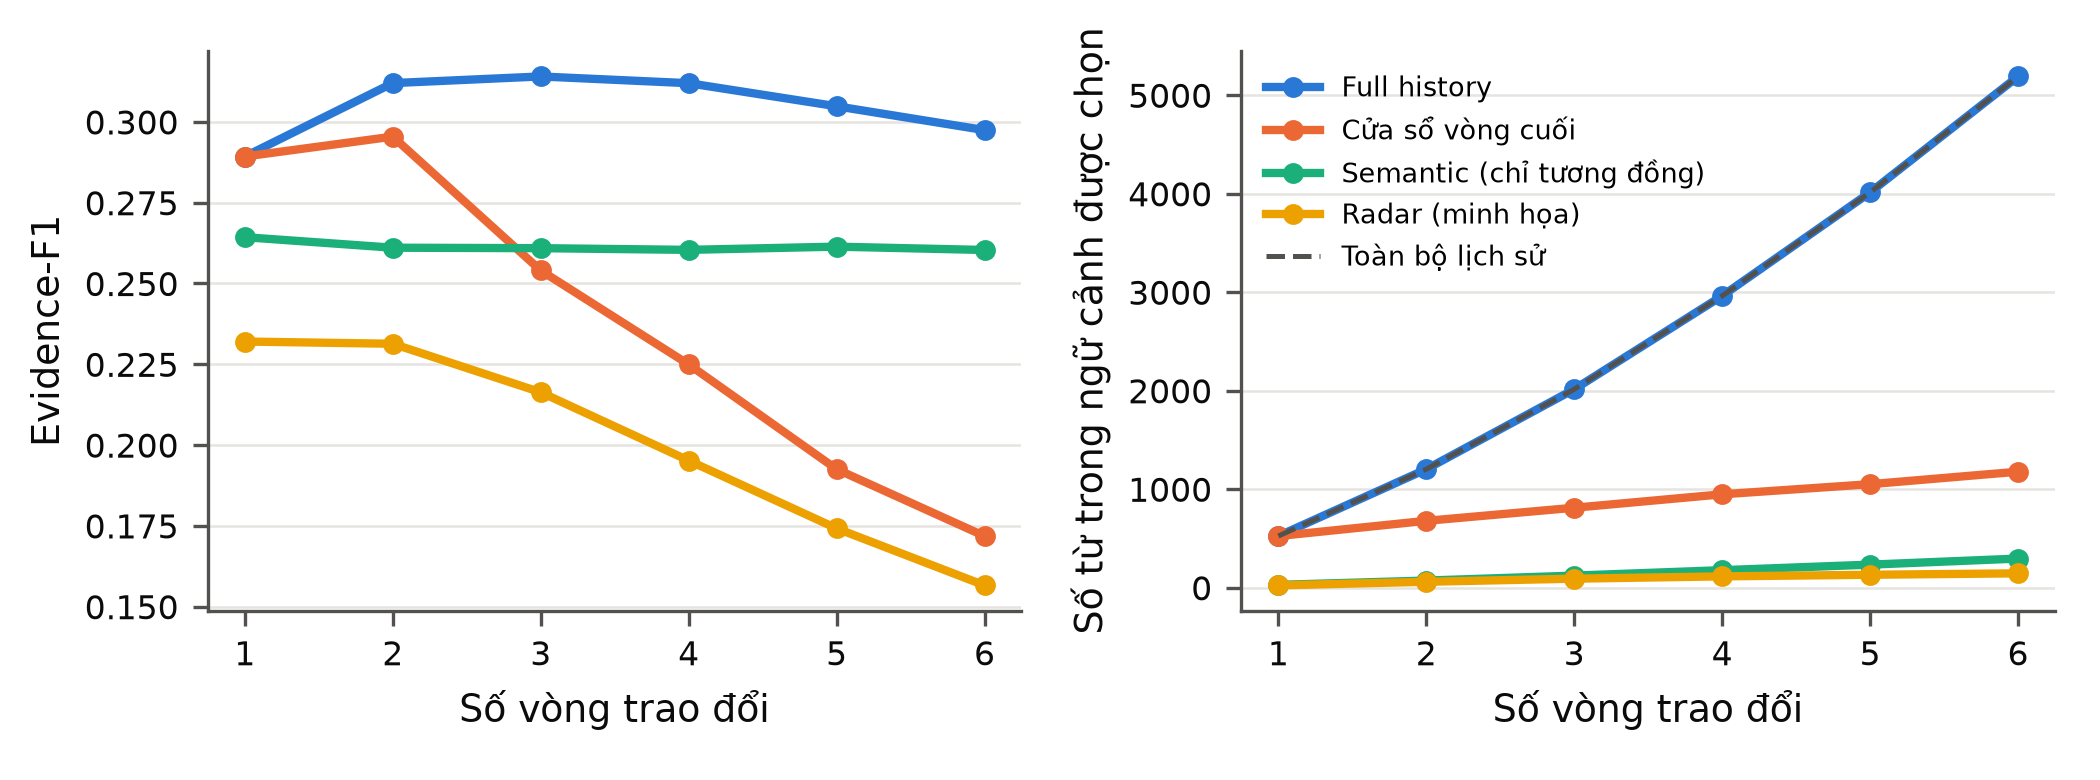
\includegraphics[width=\linewidth]{figures/exp1_rounds.png}
\caption{Thí nghiệm 1 theo số vòng trao đổi (200 mẫu HotpotQA, 5 tác tử). Trái: Evidence-F1 của ngữ cảnh được chọn so với supporting facts. Phải: số từ trong ngữ cảnh được chọn so với toàn bộ lịch sử (nét đứt). Số liệu do chương trình của báo cáo đo.}
\label{fig:exp1-rounds}
\end{figure}

Bảng~\ref{tab:exp1-rounds} và hình~\ref{fig:exp1-rounds} cho thấy ba điều. Thứ nhất, hiện tượng pha loãng xuất hiện đúng như paper mô tả: với chiến lược \texttt{full}, lịch sử phình từ 524 lên 5190 từ khi $T$ tăng từ 1 đến 6, precision của bằng chứng trong lịch sử giảm dần (từ 0,171 xuống 0,177 sau khi qua đỉnh), và Evidence-F1 đi ngang rồi giảm. Thứ hai, hai chiến lược lọc theo ngưỡng nén ngữ cảnh mạnh (radar giữ 146 từ trên 5190 từ lịch sử ở $T{=}6$, tỷ lệ $\approx$ 2,8\%) và tăng precision gấp khoảng đôi (0,33 so với 0,18), nhưng cái giá là recall: \texttt{radar} chỉ giữ lại 11\% bằng chứng vàng ở $T{=}6$. Thứ ba, chỉ số answer-acc của bộ ghép từ vựng đơn giản giảm rõ khi chuyển từ ngữ cảnh đầy đủ (0,965--0,980) sang ngữ cảnh lọc chặt (0,870--0,890).

Điểm thứ ba đáng dừng lại vì nó như là hình ảnh phản chiếu của một kết quả ablation trong paper gốc: Agent-Radar thử bỏ phần lái attention (chỉ nối các câu được chọn vào prompt) và thấy MuSiQue giảm từ 39,72 xuống 35,27 -- chọn ngữ cảnh thôi là chưa đủ. Thí nghiệm của báo cáo này không có bước lái attention (vì không chạy LLM), nên \texttt{radar} ở đây tương đương với đúng biến thể ablation đó: bộ chọn hoạt động đúng công thức, nhưng khi dùng như bộ lọc cứng thì mọi thông tin bị lọc bỏ là mất hẳn, và một bộ đọc yếu không bù lại được. Điều này củng cố thiết kế của paper gốc: giữ nguyên lịch sử và chỉ khuếch đại attention, thay vì xóa.

So trực tiếp \texttt{radar} với \texttt{semantic} (cùng ngưỡng $\theta=0{,}65$): hai hệ số suy giảm làm volume được chọn nhỏ đi (146 so với 295 từ ở $T{=}6$) nhưng không tăng precision, mà còn giảm recall (0,111 so với 0,221). Nguyên nhân nằm ở môi trường mô phỏng: nhiễu được phân bổ đều giữa các tác tử và thậm chí dày hơn ở các vòng sau (số câu nhiễu tăng theo $t$), nên vị trí không gian/thời gian ở đây hầu như không mang thông tin về chất lượng của câu -- suy giảm theo hop và theo tuổi chỉ ``trừ điểm'' thêm cho cosine. Trong hệ MAS thật mà paper xét, thông điệp xa và cũ ít đáng tin hơn, và đó là điều kiện để hai hệ số này phát huy tác dụng; môi trường mô phỏng đơn giản của báo cáo không tái tạo được điều kiện đó.

Thí nghiệm 1b kiểm chứng riêng vai trò \emph{xếp hạng} của hai hệ số suy giảm bằng cách cho mọi chiến lược chọn đúng $k$ câu (loại bỏ yếu tố ngưỡng). Kết quả: ở mọi mức $k \in \{10, 20, 40\}$, Evidence-F1 của xếp hạng có suy giảm thấp hơn chút ít so với xếp hạng thuần ngữ nghĩa (0,481 so với 0,495 tại $k{=}10$; 0,569 so với 0,584 tại $k{=}20$) -- cũng là hệ quả của việc vị trí không mang thông tin trong mô phỏng. Ngược lại, answer-acc ở $k{=}40$ nghiêng về \texttt{radar} (0,810 so với 0,785): tập được chọn ít trùng lặp hơn nên bộ ghép từ vựng nhận diện đáp án tốt hơn. Hai chiều đo cho hai kết quả khác dấu -- đây là chi tiết trung thực cần báo cáo thay vì chọn lọc cái thuận lợi.

\begin{figure}[t]
\centering
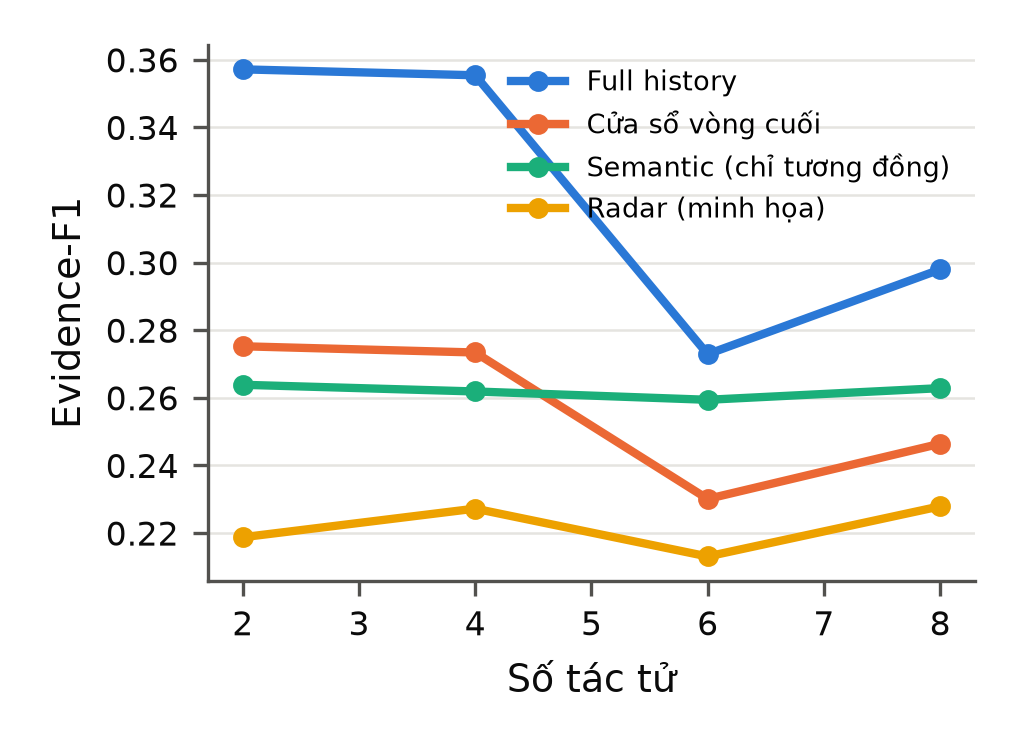
\includegraphics[width=\linewidth]{figures/exp1_agents.png}
\caption{Thí nghiệm 1 theo số tác tử ($T{=}3$). Evidence-F1 của \texttt{full} giảm khi thêm tác tử (pha loãng), còn các chiến lược lọc theo ngưỡng ổn định. Số liệu do chương trình của báo cáo đo.}
\label{fig:exp1-agents}
\end{figure}

Theo số tác tử (hình~\ref{fig:exp1-agents}), Evidence-F1 của \texttt{full} giảm từ 0,357 (2 tác tử) xuống 0,273 (6 tác tử) rồi hơi phục hồi (0,298 ở 8 tác tử) -- xu hướng ``thêm tác tử thì loãng hơn'' phù hợp với hiện tượng paper gốc mô tả ở Figure 2. Các chiến lược lọc theo ngưỡng gần như phẳng vì chúng chấm điểm theo truy vấn chứ không theo số nguồn. Thời gian chọn ngữ cảnh rất nhỏ ở mọi chiến lược (dưới 0,1 giây mỗi mẫu trên CPU; phần lớn thời gian thuộc về mã hóa câu), nên chi phí của bộ chọn không phải rào cản ở quy mô này.

\subsection{Thí nghiệm 2: DAIN đơn giản hóa trên ENRICO}

\begin{table}[t]
\centering
\caption{Thí nghiệm 2 -- accuracy trên tập test ENRICO (292 mẫu, 20 lớp; trung bình $\pm$ độ lệch chuẩn qua 5 seed, cấu hình huấn luyện giống §4.1 paper DAIN). $\bar{\tau}$: số tác tử kích hoạt trung bình; $\bar{\rho}$: mật độ đồ thị giao tiếp. Số liệu do chương trình của báo cáo đo.}
\label{tab:exp2-main}
\begin{tabular}{l rr r}
\toprule
Mô hình & Accuracy (\%) & $\bar{\tau}$/8 & $\bar{\rho}$ \\
\midrule
Early Fusion & \textbf{42,81} $\pm$ 0,57 & -- & -- \\
Late Fusion  & 41,58 $\pm$ 1,07 & -- & -- \\
Static MoE   & 39,79 $\pm$ 1,52 & 8,0 & -- \\
Sparse MoE   & 38,56 $\pm$ 1,69 & 4,0 & -- \\
DAIN-Static  & 35,14 $\pm$ 1,94 & 8,0 & 0,434 \\
DAIN-NoComm  & 37,81 $\pm$ 0,93 & 4,0 & 0,308 \\
DAIN (full)  & 38,56 $\pm$ 1,26 & 4,0 & 0,389 \\
\bottomrule
\end{tabular}
\end{table}

\begin{figure}[t]
\centering
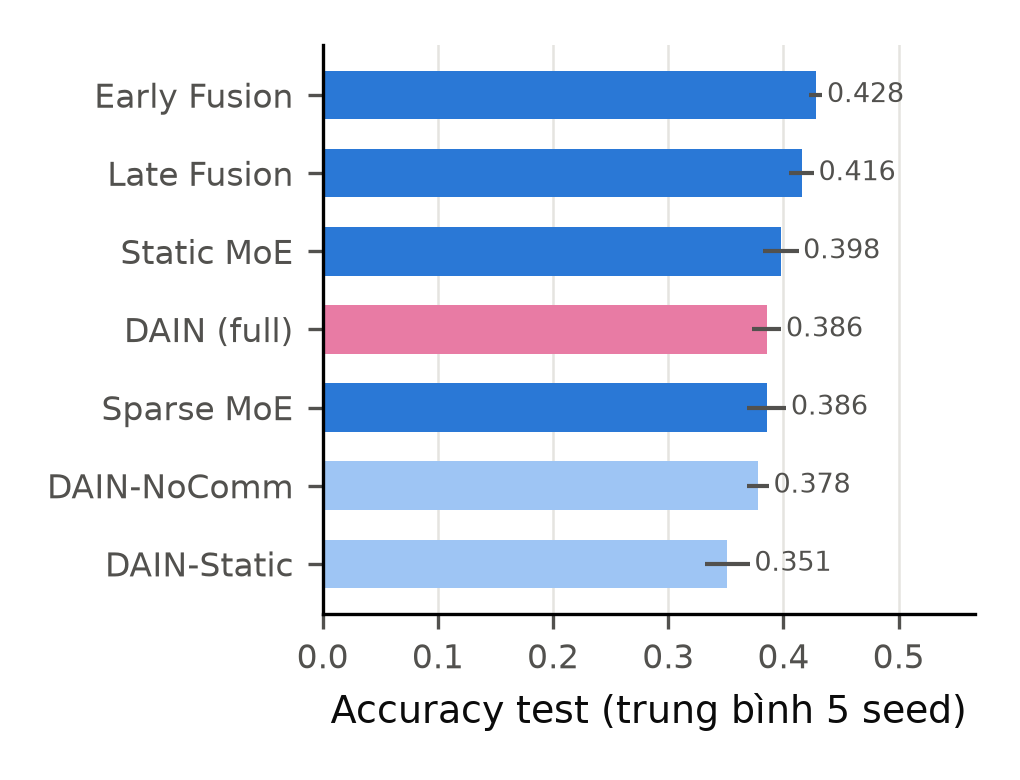
\includegraphics[width=\linewidth]{figures/exp2_main.png}
\caption{Thí nghiệm 2: accuracy trung bình qua 5 seed (thanh lỗi: độ lệch chuẩn). Ba biến thể DAIN dùng màu khác nhóm baseline để dễ theo dõi thứ tự ablation. Số liệu do chương trình của báo cáo đo.}
\label{fig:exp2-main}
\end{figure}

Bảng~\ref{tab:exp2-main} và hình~\ref{fig:exp2-main} cho kết quả chia làm hai lớp. Trong nội bộ họ DAIN, thứ tự ablation khớp định tính với Table~4 của paper: mô hình đầy đủ (38,56\%) cao hơn biến thể bỏ giao tiếp (37,81\%), và cao rõ rệt hơn biến thể mọi tác tử luôn bật (35,14\%). Cơ chế điều phối cũng hoạt động đúng thiết kế: gate giữ đúng 4/8 tác tử kích hoạt, mật độ đồ thị giao tiếp $\bar{\rho} = 0{,}39$ thấp hơn đáng kể mức dày đặc (1,0), tức Meta-Controller tự tạo ra được cấu trúc thưa như paper mô tả.

Ngược lại, lợi thế của DAIN so với các baseline fusion tĩnh -- kết quả trung tâm của paper gốc -- \emph{không} xuất hiện trong thiết lập này: Early Fusion đơn giản dẫn đầu với 42,81\%. Mức chênh vượt quá một độ lệch chuẩn của các mô hình DAIN. Một thử nghiệm chẩn đoán với learning rate cao hơn (3e-4 và 1e-3) không thay đổi thứ tự này. Có ba nguyên nhân khả dĩ, đều nằm ở những gì báo cáo phải đơn giản hóa: (i) dữ liệu nhỏ (1022 mẫu train) khiến các thành phần phụ thêm của DAIN -- 8 nhánh agent, đồ thị giao tiếp, loss chuyên môn hóa -- trở thành nguồn quá khớp hơn là lợi thế; (ii) encoder nhẹ (CNN nhỏ + bag-of-words) làm các modality ít giàu thông tin hơn nhiều so với ResNet-50/BERT-base mà paper dùng, trong khi cơ chế synergy/uniqueness/redundancy của DAIN được thiết kế để khai thác tương tác giàu giữa các modality; (iii) kết quả của paper là trung bình trên năm bộ dữ liệu với encoder chuẩn hóa, trong khi báo cáo này chỉ chạy một bộ. Nói cách khác, thí nghiệm này xác nhận kiến trúc huấn luyện được và các cơ chế điều phối vận hành đúng, nhưng không xác nhận được tuyên bố hiệu năng của paper -- và báo cáo ghi nhận điều đó nguyên văn như vậy.

\begin{figure}[t]
\centering
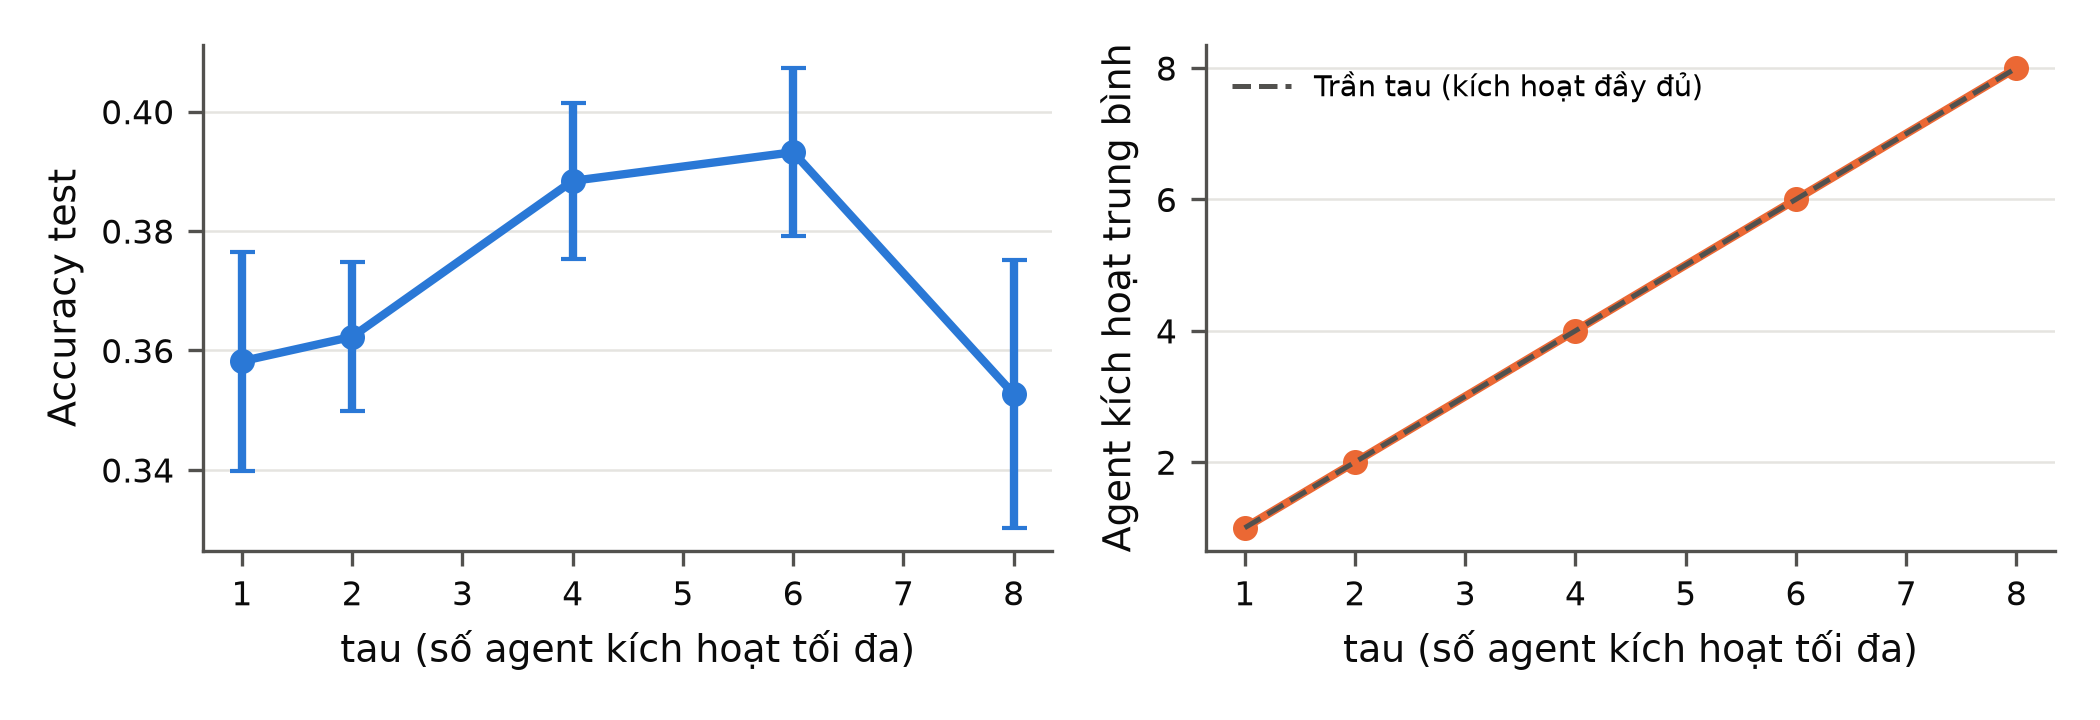
\includegraphics[width=\linewidth]{figures/exp2_tau.png}
\caption{Thí nghiệm 2: quét $\tau$ cho DAIN (trái: accuracy; phải: số tác tử kích hoạt trung bình so với trần $\tau$). Hiệu quả không đơn điệu theo $\tau$. Số liệu do chương trình của báo cáo đo.}
\label{fig:exp2-tau}
\end{figure}

Quét $\tau$ (hình~\ref{fig:exp2-tau}) cho kết quả không đơn điệu: accuracy tăng từ 35,82\% ($\tau{=}1$) lên đỉnh 39,32\% ($\tau{=}6$) rồi tụt xuống 35,27\% khi bật đủ 8 tác tử. Xu hướng ``quá ít tác tử thì thiếu, quá nhiều thì nhiễu'' khớp định tính với Table~5 của paper (đỉnh ở $\tau{=}4$, giảm nhẹ ở $\tau{=}8$), dù vị trí đỉnh khác đi -- một khác biệt nữa có thể quy về quy mô dữ liệu và encoder.

\subsection{Đối chiếu với paper gốc và giới hạn}
Tổng hợp lại: những gì hai thí nghiệm xác nhận được là (1) công thức chọn ngữ cảnh của Agent-Radar hoạt động đúng như mô tả và nén ngữ cảnh với mật độ bằng chứng cao gấp đôi baseline; (2) kết luận của paper rằng ``chọn ngữ cảnh phải đi kèm cơ chế đưa vào lúc suy luận'' thể hiện ngay cả trong một mô phỏng không có LLM; (3) thứ tự ablation của DAIN (full $>$ NoComm $>$ Static) và tính chất không đơn điệu theo $\tau$ tái hiện được ở quy mô nhỏ. Những gì không xác nhận được: lợi thế của DAIN so với baseline tĩnh trong thiết lập đơn giản hóa, và lợi thế của hai hệ số suy giảm trong môi trường mô phỏng nơi vị trí không mang thông tin. Các giới hạn khác đã nêu ở phần~\ref{sec:experiments}: thí nghiệm 1 là mô phỏng quy tắc chứ không phải hành vi LLM; thí nghiệm 2 thay encoder lớn và chỉ dùng 1/5 số bộ dữ liệu; và cả hai paper đều chưa có mã nguồn chính thức để đối chiếu.

\section{Kết luận}\label{sec:conclusion}

Báo cáo đã tìm hiểu hai công trình tiếp cận vấn đề phối hợp đa tác tử từ hai phía. Agent-Radar quản lý \emph{thông tin} trong giao tiếp: thay vì nén hoặc cắt lịch sử trao đổi, nó chấm điểm từng câu theo độ liên quan ngữ nghĩa nhân với suy giảm theo khoảng cách trên đồ thị và theo thời gian, rồi lái attention của LLM về phần được chọn. DAIN quản lý \emph{thành phần} tham gia suy luận: một Meta-Controller kích hoạt thưa nhóm tác tử chuyên biệt theo từng mẫu đa phương thức và điều phối trao đổi nén giữa chúng, huấn luyện end-to-end với loss đa mục tiêu. Điểm gặp nhau của hai thiết kế là lựa chọn phụ thuộc ngữ cảnh và sử dụng cấu trúc liên kết như một tín hiệu về độ tin cậy của thông tin; điểm khác cơ bản là một bên là lớp phủ training-free lúc suy luận, một bên là kiến trúc học từ đầu.

Phần thực nghiệm kiểm chứng được những gì tài nguyên cho phép. Với Agent-Radar, các công thức chọn ngữ cảnh được hiện thực đúng và đo được trên HotpotQA: bộ chọn giữ lại bằng chứng với mật độ cao hơn hẳn so với dùng cả lịch sử, với số token nhỏ hơn hàng chục lần; đồng thời thí nghiệm cũng cho thấy khi cơ chế chọn được dùng như bộ lọc cứng (không có bước lái attention trên toàn bộ lịch sử như paper gốc), chất lượng trả lời của một bộ đọc yếu giảm xuống -- kết quả này trái chiều với trục chính của paper nhưng nhất quán với lập luận của chính paper rằng chọn ngữ cảnh phải đi kèm cách đưa nó vào lúc suy luận. Với DAIN, bản đơn giản hóa huấn luyện được trên dữ liệu thật ENRICO và tái hiện đúng thứ tự ablation trong paper (mô hình đầy đủ tốt hơn biến thể bỏ giao tiếp, rồi đến biến thể bỏ điều phối); tuy nhiên với dữ liệu nhỏ và encoder nhẹ, mức tăng của DAIN so với early fusion trong paper chưa xuất hiện trong thiết lập của chúng tôi.

Những giới hạn còn tồn tại cần nói rõ. Thí nghiệm 1 là mô phỏng lịch sử trao đổi bằng quy tắc, không phải hành vi của LLM; môi trường mô phỏng cũng không tái tạo được tương quan giữa vị trí không gian/thời gian và độ tin cậy của thông tin -- chính yếu tố mà hai hệ số suy giảm của Agent-Radar dựa vào để phát huy tác dụng. Thí nghiệm 2 thay encoder lớn bằng encoder nhẹ và chỉ chạy một trong năm bộ dữ liệu, nên số liệu không so sánh trực tiếp với paper. Cả hai paper đều chưa công bố mã nguồn để đối chiếu từng dòng. Hướng phát triển tự nhiên tiếp theo là chạy phần lái attention (SPA) trên một LLM cục bộ nhỏ để khép lại vòng đánh giá cho Agent-Radar, và mở rộng thí nghiệm DAIN sang bộ dữ liệu thứ hai với encoder mạnh hơn.


\bibliographystyle{IEEEtran}
\bibliography{references}

\end{document}
